\documentclass[11pt,a4paper]{article}

\usepackage[utf8]{inputenc}
\usepackage[T1]{fontenc}
\usepackage{lmodern}
\usepackage[margin=2.35cm]{geometry}
\usepackage{graphicx}
\usepackage{booktabs}
\usepackage{tabularx}
\usepackage{longtable}
\usepackage{float}
\usepackage{enumitem}
\usepackage{xcolor}
\usepackage{hyperref}
\usepackage{fancyhdr}
\usepackage{tikz}
\usetikzlibrary{arrows.meta,positioning,shapes.geometric}

\hypersetup{colorlinks=true,linkcolor=blue!55!black,urlcolor=blue!55!black,citecolor=blue!55!black,pdftitle={Zombie House 3D Final Report}}
\setlength{\parindent}{0pt}
\setlength{\parskip}{0.45em}
\setlist{nosep}
\renewcommand{\arraystretch}{1.18}

\pagestyle{fancy}
\fancyhf{}
\lhead{CS427 - 3D Visualization and Game Development}
\rhead{Zombie House 3D}
\cfoot{\thepage}
\setlength{\headheight}{14pt}

\begin{document}
\pagenumbering{gobble}
\begin{titlepage}
\begin{tikzpicture}[remember picture,overlay]
  \draw[blue!65!black,line width=3pt]
    ([xshift=1.5cm,yshift=-1.5cm]current page.north west) rectangle
    ([xshift=-1.5cm,yshift=1.5cm]current page.south east);
\end{tikzpicture}
\begin{center}
  \vspace*{0.8cm}
  {\large\textbf{VNUHCM - UNIVERSITY OF SCIENCE}}\\[4pt]
  {\large\textbf{ADVANCED PROGRAM IN COMPUTER SCIENCE}}\\[1.2cm]
  
\includegraphics[width=0.24\textwidth]{../template-report/logo-khtn.png}\\[1.15cm]
  {\Huge\textbf{ZOMBIE HOUSE 3D}}\\[0.35cm]
  {\Large Final Project Report}\\[1.35cm]
  {\Large\textbf{CS427 - 3D Visualization and Game Development}}\\[1.2cm]
\end{center}

\begin{tabularx}{\textwidth}{@{}lX@{}}
\textbf{Lecturer:} & Assoc. Prof. Dr. Tran Minh Triet\\[5pt]
\textbf{Teaching Assistant:} & Tran Ngoc Dat Thanh\\[5pt]
\textbf{Project team:} & Huynh Tran Uy - 23125047\\
& Tran My An - 23125049\\
& Nguyen Hoang Gia Han - 23125055\\
& Pham Bao Kha - 23125058\\
\end{tabularx}

\vfill
\begin{center}
  \large September 2026
\end{center}
\end{titlepage}

\clearpage
\pagenumbering{arabic}
\tableofcontents
\newpage

\section{Introduction and Game Concept}

\textit{Zombie House 3D} is a third-person, low-poly 3D defense game. The player protects a house from advancing zombie waves by positioning defensive plants, fighting nearby enemies, and managing limited resources. The project combines a readable stylized world with a compact survival loop: prepare a lane, react to enemies, protect the base, and clear all waves.

The game is designed for short sessions and clear feedback. A round is won when all configured waves are defeated; it is lost when the house health reaches zero. Three visual map variants---day, cloudy, and night---support the same core game idea while giving the project a stronger presentation layer.

\textbf{Design goals.} The project is guided by three practical goals:
\begin{itemize}
  \item Make the defense objective immediately understandable through the house, lanes, enemies, health state, and round UI.
  \item Combine direct player action with strategic plant placement instead of relying on a purely passive tower-defense experience.
  \item Use a modular Unity scene and prefab structure so maps, waves, plants, enemies, and UI can be iterated independently.
\end{itemize}

\section{Gameplay and Player Experience}

\subsection{Core loop}
At the start of a round, the player enters a protected area containing planting lanes and a house objective. Sun is collected and spent to deploy plants on valid squares. Zombies enter through configured routes and move toward the house. Plants automatically engage targets in their lane while the player can move, attack, plant, and remove plants. The player adapts the defense until every wave is cleared or the base is destroyed.

\begin{figure}[H]
\centering
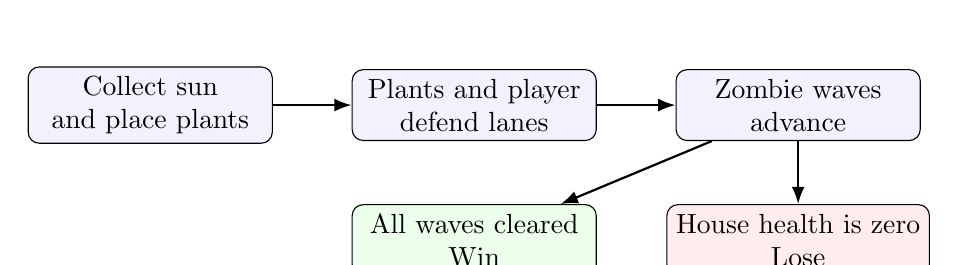
\begin{tikzpicture}[
  node distance=8mm and 10mm,
  box/.style={draw,rounded corners,align=center,minimum width=31mm,minimum height=9mm,fill=blue!5},
  arrow/.style={-{Latex[length=2.2mm]},thick}
]
\node[box] (prepare) {Collect sun\\and place plants};
\node[box,right=of prepare] (defend) {Plants and player\\defend lanes};
\node[box,right=of defend] (waves) {Zombie waves\\advance};
\node[box,below=of defend,fill=green!8] (win) {All waves cleared\\Win};
\node[box,below=of waves,fill=red!7] (lose) {House health is zero\\Lose};
\draw[arrow] (prepare)--(defend);
\draw[arrow] (defend)--(waves);
\draw[arrow] (waves)--(win);
\draw[arrow] (waves)--(lose);
\end{tikzpicture}
\caption{High-level gameplay loop.}
\end{figure}

\subsection{Controls and feedback}
The player uses standard third-person movement and camera control. Contextual actions cover selecting a plant, placing it on a free planting square, removing a placed plant, and melee attacking nearby zombies. The UI presents the active round, resource state, base health, and win/lose outcome. Audio reinforces menu navigation, attacks, plant placement, projectile hits, zombie events, resource collection, and round results.

\subsection{Tutorial map requirement}
The next user-facing addition is a dedicated instruction map. It will teach movement, camera control, plant selection and placement, melee attacks, plant removal, resource collection, and the win/loss objective in a safe sequence before the player enters a full round.

\section{Technical Implementation}

\subsection{Technology stack}
\begin{tabularx}{\textwidth}{>{\bfseries}p{0.24\textwidth}X}
\toprule
Layer & Technology and role\\
\midrule
Game engine & Unity 6.3 LTS with Universal Render Pipeline (URP) for scene management, rendering, prefabs, physics, and UI.\\
Programming & C\# scripts for player input, combat, zombies, waves, health, economy, object pooling, UI state, and audio.\\
Input and UI & Unity Input System and Unity UI for character selection, round selection, HUD, and win/lose panels.\\
Version control & Git and GitHub branches for parallel feature development and integration.\\
Assets & Unity Asset Store packages, KayKit characters, a Cartoon Zombie model, and documented third-party audio.\\
\bottomrule
\end{tabularx}

\subsection{Runtime structure}
The project separates reusable gameplay systems from map presentation. The main menu selects a round and loads a map scene. Gameplay scenes contain the player, routes, planting area, house target, spawner, grid, and UI systems. Managers coordinate economy, waves, game state, and object pooling, while prefabs keep plants and enemy types reusable.

\begin{figure}[H]
\centering
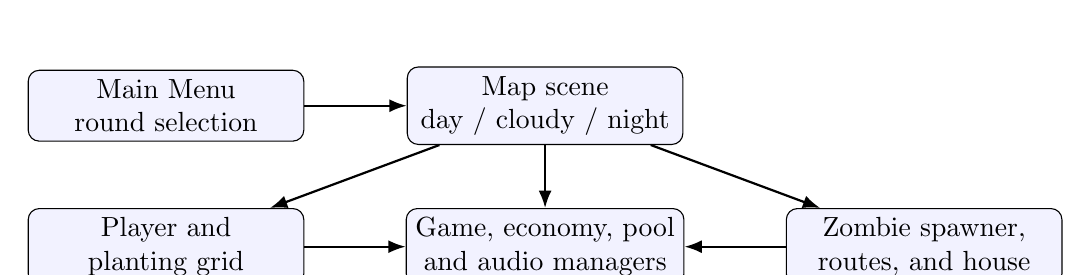
\begin{tikzpicture}[
  node distance=8mm and 13mm,
  box/.style={draw,rounded corners,align=center,minimum width=35mm,minimum height=9mm,fill=blue!5},
  arrow/.style={-{Latex[length=2.2mm]},thick}
]
\node[box] (menu) {Main Menu\\round selection};
\node[box,right=of menu] (map) {Map scene\\day / cloudy / night};
\node[box,below left=of map] (player) {Player and\\planting grid};
\node[box,below=of map] (manager) {Game, economy, pool\\and audio managers};
\node[box,below right=of map] (enemy) {Zombie spawner,\\routes, and house};
\draw[arrow] (menu)--(map);
\draw[arrow] (map)--(player);
\draw[arrow] (map)--(manager);
\draw[arrow] (map)--(enemy);
\draw[arrow] (player)--(manager);
\draw[arrow] (enemy)--(manager);
\end{tikzpicture}
\caption{Scene-level organization of the game.}
\end{figure}

\subsection{Audio service}
A persistent \texttt{AudioManager} selects menu music for \texttt{MainMenu} and gameplay music for map scenes. It exposes named one-shot cues for UI and gameplay events and uses several SFX sources so concurrent sounds do not cut each other off. A fallback Audio Listener supports isolated test scenes that do not have a camera.

\section{Key Game Features}

\begin{figure}[H]
  \centering
  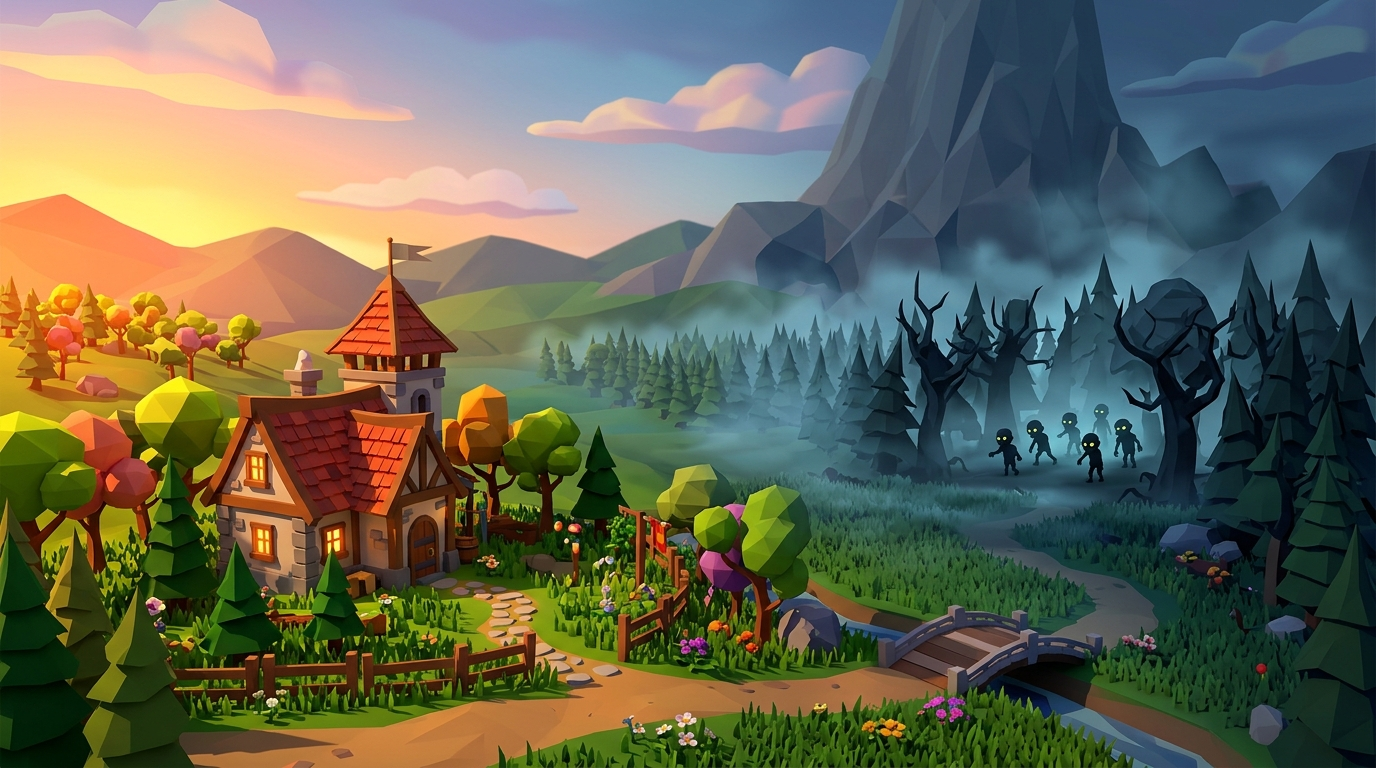
\includegraphics[width=\textwidth]{images/main-menu-visual.jpg}
  \caption{Project visual used for the main-menu presentation: a protected house facing an approaching zombie threat.}
  \label{fig:main-menu-visual}
\end{figure}

\textit{Zombie House 3D} is designed around readable, complementary systems rather than a large number of unrelated mechanics. Figure~\ref{fig:main-menu-visual} communicates the intended contrast between the player's safe base and the hostile enemy area; the following features turn that setting into a playable defense round.

\subsection{Player-driven combat and planting}
\begin{itemize}
  \item \textbf{Third-person movement and melee:} the player can move around the map, adjust the camera, and fight enemies that reach the defensive line.
  \item \textbf{Plant-based defense:} plantable squares and plant data allow the player to place defenders deliberately instead of depending only on direct attacks.
  \item \textbf{Resource decisions:} the sun economy connects resource collection and plant costs, requiring the player to decide when and where to invest in defense.
  \item \textbf{Flexible interaction:} selected plants can be placed or removed, which supports correction and adaptation during a round.
\end{itemize}

\subsection{Enemy waves, progression, and feedback}
\begin{itemize}
  \item \textbf{Wave defense:} zombies follow routes toward the house, attack when they arrive, and are cleared through coordinated player and plant damage.
  \item \textbf{Multiple enemy forms:} the integration setup includes standard zombie behavior and a spider/zombie variant, making the enemy system extensible.
  \item \textbf{Clear game states:} house health, wave progression, and win/lose panels communicate whether the player is holding the defense or has completed the round.
  \item \textbf{Presentation support:} day, cloudy, and night map variants, a minimap, menu navigation, background music, and action SFX reinforce orientation and feedback.
\end{itemize}

\begin{figure}[H]
  \centering
  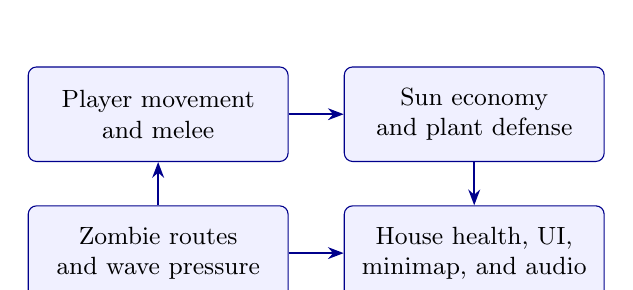
\begin{tikzpicture}[
    node distance=0.55cm and 0.7cm,
    feature/.style={draw=blue!55!black, rounded corners=3pt, fill=blue!6, minimum width=3.3cm, minimum height=1.2cm, align=center, font=\small},
    flow/.style={-{Stealth[length=2mm]}, thick, blue!55!black}
  ]
    \node[feature] (player) {Player movement\\and melee};
    \node[feature, right=of player] (plants) {Sun economy\\and plant defense};
    \node[feature, below=of player] (waves) {Zombie routes\\and wave pressure};
    \node[feature, below=of plants] (feedback) {House health, UI,\\minimap, and audio};
    \draw[flow] (player) -- (plants);
    \draw[flow] (plants) -- (feedback);
    \draw[flow] (waves) -- (player);
    \draw[flow] (waves) -- (feedback);
  \end{tikzpicture}
  \caption{The main gameplay features form one defense loop: enemy pressure drives player and plant actions, while the house and UI provide the round's feedback.}
  \label{fig:feature-loop}
\end{figure}

\section{Game Features}

\begin{longtable}{p{0.30\textwidth}p{0.63\textwidth}}
\toprule
Feature & Description\\
\midrule
Main menu and round flow & Character and round selection route the player to the available map scenes.\\
Map presentation & Day, cloudy, and night variants provide the project's low-poly outdoor setting.\\
Player interaction & Third-person movement, camera control, melee attack, plant selection, placement, and removal support direct interaction during a round.\\
Plants and economy & Plant data, sun economy, planting squares, and Peashooter projectile combat form the defense layer.\\
Zombie gameplay & Route movement, health, melee attacks, waves, a house target, and spider/zombie enemy variants define the enemy challenge.\\
Minimap & The minimap follows the player and identifies zombies, helping players remain oriented in the main maps.\\
Win/lose UI & Result panels and their associated logic communicate the outcome of each round.\\
Audio & Dedicated menu and gameplay background music, plus UI, combat, plant, zombie, house, resource, and result sound effects support feedback.\\
Tutorial map & A guided instruction map introduces movement, planting, attacking, plant removal, resource collection, and the defense objective.\\
\bottomrule
\end{longtable}

Together, these features establish a complete 3D defense-game loop from menu selection to the final win or lose result.

\clearpage
\section{Team Contributions and Remaining Work}

\begin{longtable}{p{0.24\textwidth}p{0.18\textwidth}p{0.48\textwidth}}
\toprule
Member & Student ID & Main contribution\\
\midrule
Huynh Tran Uy & 23125047 & Core gameplay development: player combat, zombie behavior, wave/gameplay integration, and reusable gameplay systems.\\
Tran My An & 23125049 & Visual map variants, menu and character-selection UI, and enhancement of the win/lose presentation and round flow.\\
Nguyen Hoang Gia Han & 23125055 & Map-route integration support, project audio service and sound library, asset/setup investigation, quality checks, and report preparation.\\
Pham Bao Kha & 23125058 & Minimap implementation, project organization, and integration of plantable squares into the map.\\
\bottomrule
\end{longtable}

\textbf{Immediate roadmap.} The remaining work is organized around a complete, testable game flow:
\begin{enumerate}
  \item Integrate plantable squares, minimap, house, waves, and enhanced win/lose UI into the principal round maps as one verified gameplay flow.
  \item Create a tutorial/instruction map covering movement, planting, attacking, removing plants, resource collection, and objectives.
  \item Balance wave counts, plant costs, enemy health, and sound volumes after repeated playtests.
  \item Run a final scene-by-scene regression test from Main Menu to win/lose outcomes and verify all third-party asset credits.
\end{enumerate}

\section{Conclusion}

Zombie House 3D establishes a playable 3D defense-game foundation in Unity: an explorable low-poly setting, round selection, direct player combat, plant-based defense, routed enemies, base health, UI feedback, and an audio layer. The next milestone is not a new game concept but a focused integration pass: place the remaining gameplay systems in the main maps, add the tutorial scene, and tune the complete loop through playtesting. This approach keeps the project achievable while producing a coherent final player experience.

\begin{thebibliography}{9}
\bibitem{unity} Unity Technologies, \emph{Unity Manual and Scripting API}. \url{https://docs.unity3d.com/}.
\bibitem{input} Unity Technologies, \emph{Input System package documentation}. \url{https://docs.unity3d.com/Packages/com.unity.inputsystem@latest}.
\bibitem{urp} Unity Technologies, \emph{Universal Render Pipeline documentation}. \url{https://docs.unity3d.com/Manual/com.unity.render-pipelines.universal.html}.
\bibitem{assets} Project team, \emph{ASSETS.md: Third-Party Assets}, project repository, accessed September 2026.
\bibitem{kaykit} KayKit Game Assets, \emph{KayKit Character Pack Adventures}. \url{https://github.com/KayKit-Game-Assets/KayKit-Character-Pack-Adventures-1.0}.
\bibitem{zombie} Vinrax, \emph{Cartoon Zombie}, CC-BY 3.0; attribution retained in the project asset folder.
\bibitem{audio-menu} TAD, \emph{Once Upon a Time (loop)}, CC0. \url{https://opengameart.org/content/once-upon-a-time-loop}.
\bibitem{audio-game} request, \emph{Heartfelt Battle (loopable fantasy music)}, CC0. \url{https://opengameart.org/content/heartfelt-battle-loopable-fantasy-stringspianohorn}.
\bibitem{kenney} Kenney, \emph{Interface Sounds} and \emph{RPG Audio}, CC0. \url{https://kenney.nl/assets/interface-sounds}; \url{https://kenney.nl/assets/rpg-audio}.
\end{thebibliography}

\end{document}
